\section{Security Model}
\subsection{Taxonomy of Timing Channels}
    \begin{figure}
        \begin{center}
            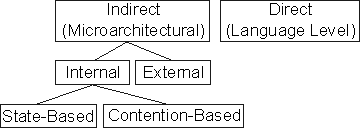
\includegraphics[width=2.6in]{figs/taxonomy.pdf}
            \caption{The taxonomy of timing channels}
            \label{fig:taxonomy}
        \end{center}
    \end{figure}

A timing channel is a vulnerability that correlates secret data with the  
timing of events within a system thereby forming a channel for communicating or 
extracting secret data despite the intentions of the system designer. Figure 
\ref{fig:taxonomy} summarizes the taxonomy of timing channels. \emph{Direct} or 
software visible timing channels can be identified by examining the source code 
\cite{mitigation3}. A password checking algorithm that stops as soon as an 
incorrect character is found causes a direct timing channel that leaks 
information about the correct password. In contrast, \emph{indirect} or 
microarchitectural timing channels cannot be identified in the source code 
since they depend on hardware level behavior \cite{mitigation3}. Conventional 
caches cause an indirect timing channel whenever the probability of a cache hit 
depends on secret data. Programming language techniques have been developed to 
address software visible timing channels 
\cite{timesens,mitigation1,mitigation2,mitigation3}. It is possible to reduce 
the information leaked by some microarchitectural timing channels at the 
language level \cite{mitigation3}. However, eliminating all leakage caused by 
microarchitectural timing channels is difficult without hardware support.
%%%% More precise, wordier version:
%  However, efficiently providing strict timing-sensitive noninterference in 
%  the presence microarchitectural timing channels without the support of 
%  hardware is a hard problem.

Microarchitectural timing channels can be further divided into internal or 
external timing channels. \emph{External} timing channels are not caused by 
interference, and are exploited by an adversary that directly measures the 
timing of the victim's actions. External timing channels can be exploited by an 
adversary that does not share hardware with the victim. Bernstein's 
attack~\cite{bernstein} exploits an external timing channel in popular 
implementations of AES (such as OpenSSL). The external timing channel exists 
because the cache access pattern both affects the overall execution time of the 
AES implementation and depends on the secret key. The adversary carries out the 
attack without sharing any hardware by directly measuring the response times of 
the victim machine.
% The long explanation
% The adversary uses a copy of the same AES implementation as the victim to 
% time the encryption of a number inputs with a known key on the adversary's 
% local machine. Then, the adversary makes requests to the victim machine using 
% the same inputs and times how long the victim machine takes to encrypt the 
% inputs with an unknown key. In both cases, the execution time depends on the 
% cache access pattern which depends on the key. The adversary can use the 
% timing information gathered with the known and unknown keys to learn the 
% secret AES key.

\emph{Internal} timing channels are exploited by an adversary that shares 
hardware with the victim, and are caused by interference between the adversary 
and the victim. An adversary exploits the internal timing channel by measuring 
the timing of its own actions rather than measuring the actions of the victim 
directly. For example, an adversary can fill a cache shared with the victim, 
wait for the victim to execute, and then issue another sequence of cache 
accesses while measuring the time. Since a miss implies the victim caused a 
cache block replacement, the timing of the adversary's requests correlate with 
the victim's cache access pattern. Percival~\cite{percival} has shown that the 
S-box lookups in most common implementations of AES have an internal timing 
channel through the cache that can be used to extract cryptographic keys. 

Internal microarchitectural timing channels can either be state based, or 
contention based. In a \emph{state based} timing channel, the victim and 
adversary share some hardware state element where the time required to use that 
component depends on the state. Conventional caches shared between a victim and 
adversary have state based timing channels; accesses to memory addresses in the 
cache are faster than those that are not, and the victim's access pattern can
replace adversary cache blocks. In a \emph{contention based} timing channel, 
the victim and adversary share a resource that can handle only a finite number 
of requests at a time. Often, requests made to the resource while it is already 
handling a request are delayed. Conventional buses have contention based timing 
channels since a finite number of requests can be transferred at a time while 
the remaining requests are delayed in a queue.

%% Not sure if this
We show how this taxonomy can be used to identify general approaches to prevent 
each type of timing channel in Section \ref{sec:tc_sources}. Though the use of 
a victim and an adversary in these definitions may seem to limit this taxonomy 
to timing side channels, it is equally valid for categorizing timing covert 
channels. To categorize covert channels, the victim is replaced with an 
adversary that intentionally sends messages to a second adversary through the 
timing channel.

\subsection{Threat Model}
The goal of this work is to completely isolate distrusting software entities, 
such as threads, processes, or virtual machines that share hardware. The system 
should be no less secure than running the software entities on separate 
hardware. 

\begin{figure}
    \begin{center}
        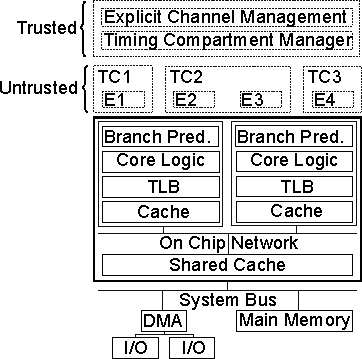
\includegraphics[width=3in]{figs/threat_model.pdf}
        \caption{The Timing Compartments threat model.}
        \label{fig:threat_model}
    \end{center}
\end{figure}

Figure \ref{fig:threat_model} shows a general hardware/software architecture on 
which we base our threat model. The hardware architecture has multiple cores, 
each with private resources such as a branch predictor, one or more private 
caches, a TLB, and the core logic. Each processor is connected to a shared 
cache through an on-chip network. The multicore processor is connected to the 
main memory and a DMA module through the system bus. The hardware is 
concurrently shared by multiple software entities. It is possible for software 
entities to be time multiplexed on the same core (e.g.  by context switching 
VMs), but the system does not allow software entities to execute concurrently 
on the same core (e.g. through simultaneous multithreading). 

We assume that conventional software isolation abstractions such as threads, 
processes, and machine virtualization along with access controls provide 
isolation through explicit channels. However, these approaches to isolate 
software do not address timing channels that leverage shared hardware. To 
guarantee total isolation, internal timing channels must also be eliminated.  
Since our goal is to make shared hardware as secure as separate hardware, 
timing channels that are external to the hardware are not addressed. Any timing 
channels that are external to the hardware in this system would also be present 
if the software entities executed on separate hardware. If necessary, external 
timing channels can be controlled in software.

Our approach to controlling timing channels is to group software entities
into a hardware/software architecture primitive called a timing compartment 
(TC) which controls timing channel leakage out of the compartment. The system 
requires a trusted software layer (see Figure \ref{threat_model}) comprised of 
the software that controls explicit channels (e.g.  the OS or hypervisor) and 
is extended to include a timing compartment manager (TCM). The TCM sets up 
these timing compartments and initializes the hardware to track actions 
performed on behalf of these timing compartments at the hardware level. Then, 
the hardware architecture controls how the timing compartments use shared 
resources to eliminate interference and provide timing channel isolation.  
Timing compartments are described in further detail in the following section.  
Intuitively, a single timing compartment contains only software entities that 
trust each other explicitly (such as all the VMs on a machine owned by the same 
user) or implicitly (all the VMs that do not want to pay for protection), 
however, timing channel leakage between entities in different timing 
compartments must be controlled. Figure \ref{threat_model} shows a system with 
4 software entities grouped into 3 timing compartments. Entities 2 and 3 trust 
each other.2 and 3 trust each other.2 and 3 trust each other. The entities in 
all timing compartments must trust the TCM, but since the TCM distrusts all 
other timing compartments, it also requires timing channel protection.

\subsection{Example Scenarios}
This section describes several application domains and scenarios that conform 
to our threat model and can be secured with timing compartments.
\subsubsection{Cloud Computing}
In platform as a service (PaaS) cloud computing, a cloud provider owns hardware 
which is shared by virtual machines that are managed by a hypervisor. The cloud 
provider leases out the virtual machines with a pre-configured software stack 
to third parties. The VMs are inexpensive since the cloud provider leverages an 
economy of scale.
However tenants in a PaaS environment have no control over the VMs they 
co-reside with; they may share hardware with competitors or attackers that want 
to extract sensitive data. One purpose of machine virtualization is to isolate 
separate OS environments, but the platform as a whole is still less secure than 
executing on separate hardware. Timing channels can violate VM isolation.
For some clients without strong security requirements, this is not a concern, 
but for others, this security threat makes cloud computing inviable.

Figure \ref{fig:cloud_scenario} shows an example cloud computing environment 
with four virtual machines with different platforms and security requirements.
VM1 runs program with high security requirements and distrusts all other VMs in 
the environment. Unfortunately, the system has microarchitectural timing 
channels (e.g. in the shared cache) that enable any coresident VM to extract 
secrets from VM1 using side channel attacks. VM2 runs an application that has 
low security requirements, but is very performance intensive. VM2 needs the 
explicit channel isolation provided by machine virtualization, but the owner 
would rather not incur performance overheads for unneeded timing channel 
protection. VM4 uses a platform containing a proprietary algorithm, AlgoX, 
owned by the cloud provider. To prevent tenants from stealing the algorithm, 
the cloud provider restricts the network usage of any tenants using AlgoX. To 
circumvent this, the owner of VM4 requests VM3 which does not use the algorithm 
(or have the network restrictions). VM4 can leak the algorithm over a covert 
channel with VM3 by exploiting microarchitectural timing channels (in the 
network on chip, for example).

